%%%%%%%%%%%%%%%%%%%%%%%%%%%%%%%%%%%%%%%%%%%%%%%%%%%%%%%%%%%%%%%%%%%%%%%%%%
%% CV-SerafinVelezVarrera 0.1, 2014-10-17				%%
%% Written by Serafín Vélez Barrera <serafa12000@gmail.com> 		%%
%% ---------------------------------------------------------- 		%%
%% Licensed under							%%
%% 	Creative Commons Attribution-NonCommercial-ShareAlike 3.0	%%
%% http://creativecommons.org/licenses/by-nc-sa/3.0/			%%
%%%%%%%%%%%%%%%%%%%%%%%%%%%%%%%%%%%%%%%%%%%%%%%%%%%%%%%%%%%%%%%%%%%%%%%%%%

%%%%%%%%%%%%%%%%%%%%%%%%%%%%%%%%%%%%%%%%%%%%%%%%%%%%%%%%%%%%%%%%%%%%%%%%%%
%				Preámbulo				 %
%%%%%%%%%%%%%%%%%%%%%%%%%%%%%%%%%%%%%%%%%%%%%%%%%%%%%%%%%%%%%%%%%%%%%%%%%%


% Definición del documento
\documentclass{beamer}
\usepackage[utf8x]{inputenc}
\usepackage[spanish]{babel}
\usepackage{beamerthemeshadow}
\usepackage{hyperref}
\usepackage{ragged2e} 
\usetheme{Antibes}
\usepackage{listings}
\setbeamercovered{transparent}
 
\usepackage{pxfonts}


% Preámbulo -> Definición del título del documento, autor, institución, fecha y fondo para las transparencias.
\title{Scraping express}
\subtitle{El arte de recuperar datos}
\author[Serafín Vélez Barrera]{Serafín Vélez Barrera\\ \scriptsize{\texttt{\href{mailto:serafa12000@gmail.com}{serafa12000@gmail.com}} -- \href{http://twiter.com/seravb}{@seravb}}}
% \date{22/01/2013}
%\institute{
\includegraphics[scale=0.5]{Imagenes/LogoOSL.png} \\ \flushright 
\includegraphics[scale=0.5, keepaspectratio=true]{Licencia/By-sa.png}}
\institute{\href{http://osl.ugr.es}{
\includegraphics[scale=0.5]{Imagenes/LogoOSL.png}} \\ \flushright \href{http://creativecommons.org/licenses/by-nc-sa/3.0/deed.es_ES}{
\includegraphics[scale=0.5, keepaspectratio=true]{Licencia/00_CreativeCommons.png}}}
\usebackgroundtemplate{
\includegraphics[width=\textwidth]{Imagenes/earth_con_opacidad.pdf}}



% Comandos personalizados
\newcommand{\negrita} % Texto en negrita
[1]{\textbf{#1}}
\newcommand{\cursiva} % Texto en cursiva
[1]{\textit{#1}}
\newcommand{\negritacursiva} % Texto en negrita-cursiva
[1]{\textbf{\textit{#1}}}


% Documento
\begin{document}
	\lstset{language=python,
        numbers=left,
        numberstyle=\tiny,
        showstringspaces=false,
        aboveskip=-40pt,
        frame=leftline
        }

	\begin{frame}
		\titlepage
	\end{frame}


	\begin{frame}
	        \frametitle{Índice}
	        \tableofcontents
	\end{frame}


	\section{Introducción}
		\begin{frame}
			\frametitle{¿Qué eso del scraping?}
			\large El scraping es un técnica que se usa para recuperar \negrita{datos} de una web o documento básicamente.
		\end{frame}
	
	\section{¿Cómo se hace?}
		\begin{frame}
			\frametitle{¿Cómo se hace?}
			Existen varios métodos, por ejemplo:
			\begin{tabular} { l | c | r }
				Para una web & Algún framework & Scrapy, FastCrawl.. \\
				Tablas de PDF & Algunas web & Tabula
			\end{tabular}
		\end{frame}


	\section{Scrapy}
		\begin{frame}
			\frametitle{Instalación de Scrapy}
				Podremos instalar Scrapy de varias maneras:
				\begin{itemize}
					\item Descarga de la \href{http://scrapy.org/}{web oficial de Scrapy}
					\item Línea de comandos:\\
						\begin{itemize}
							\item easy\_install -U Scrapy
							\item pip install Scrapy
						\end{itemize}
					\item Centro de software
				\end{itemize}
		\end{frame}
		\begin{frame}
			\frametitle{Conociendo a Scrapy}
				Cuando usamos Scrapy tenemos que crear un proyecto, y cada proyecto se compone de:
				\begin{itemize}
					\item[Items] Definimos los elementos a extraer.
					\item[Spiders] Es el corazón del proyecto, aquí definimos el procedimiento de extracción.
					\item[Pipelines] Son los elementos para analizar lo obtenido: validación de datos, limpieza del código html...
				\end{itemize}
		\end{frame}
		\begin{frame}
			\frametitle{Internamente Scrapy}
			\begin{center}
				\begin{figure}
					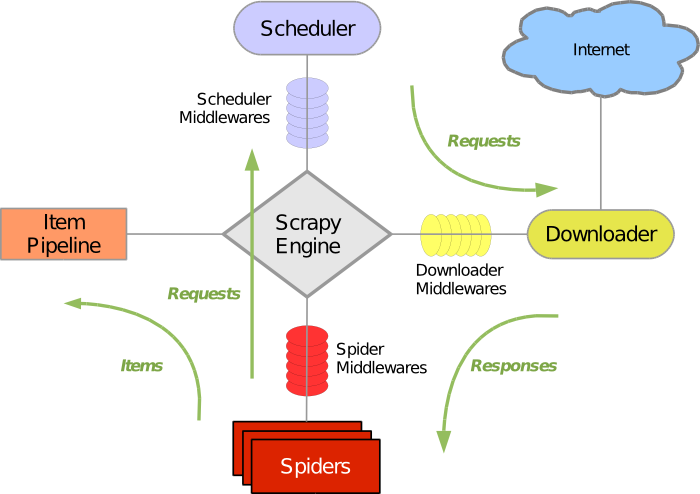
\includegraphics[keepaspectratio=true, scale=0.5]{Imagenes/scrapy_architecture.png}
				\end{figure}
			\end{center}
		\end{frame}
		\begin{frame}[fragile]
			\frametitle{Primeros pasos - Crear un proyecto}
				\begin{semiverbatim}
					\begin{lstlisting}
					scrapy startproject OpenDataDayProject
					\end{lstlisting}
				\end{semiverbatim}
		\end{frame}
		\begin{frame}[fragile]
			\frametitle{Primeros pasos - Definición de la información}
				\begin{semiverbatim}
					\begin{lstlisting}
					from scrapy.item import Item, Field
					class ODDItem(Item):
					    title = Field()
					    link = Field()
					    desc = Field()
					\end{lstlisting}
				\end{semiverbatim}
		\end{frame}
		\begin{frame}[fragile]
			\frametitle{Primeros pasos - Programación de los Spiders}
				\begin{semiverbatim}
					\begin{lstlisting}
					from scrapy.spider import BaseSpider
					class ODDSpider(BaseSpider):
					    name = "odd"
					    allowed\_domains = ["ugr.es"]
					    start\_urls = [
					        "http://www.ugr.es"
					    ]
					    def parse(self, response):
					        filename = response.url.split("/")[-2]
					        open(filename, 'wb').write(response.body)
					\end{lstlisting}
				\end{semiverbatim}
		\end{frame}
		\begin{frame}[fragile]
			\frametitle{Primeros pasos - Ejecutando el proyecto}
				\begin{semiverbatim}
					\begin{lstlisting}
					scrapy crawl OpenDataDayProject
					\end{lstlisting}
				\end{semiverbatim}
		\end{frame}
		\begin{frame}[fragile]
			\frametitle{Primeros pasos - Salvando lo obtenido}
				\begin{semiverbatim}
					\begin{lstlisting}
					scrapy crawl OpenDataDayProject -o info.json -t json
					\end{lstlisting}
				\end{semiverbatim}
		\end{frame}


	\section{Conclusiones}
		\begin{frame}
			\frametitle{Conclusión}
			\begin{enumerate}
				\item Piensa bien que quieres buscar/hacer (piensa en los aspectos legales también).
				\item Búscate algún framework para trabajar o prográmate tu script/programa para extraer datos.
				\item Extrae los datos.
				\item Procésalos.
				\item Almacénalos si te es necesario.
			\end{enumerate}
 		\end{frame}
		\begin{frame}
			\begin{center}
				
\includegraphics[height=\textheight, keepaspectratio=true]{Imagenes/PreguntasDudasAclaraciones.png}
			\end{center}
		\end{frame}

		% BIBLIOGRAFÍA
		\begin{frame}
			\frametitle{Bibliografía}
			\begin{itemize}
				\item \href{http://scrapy.org/}{Web oficial de Scrapy}
				\item \href{http://doc.scrapy.org/en/latest/intro/overview.html}{Scrapy en un vistazo}
				\item \href{http://doc.scrapy.org/en/latest/intro/tutorial.html}{Tutorial de Scrapy}
				\item \href{https://github.com/scrapy/dirbot}{Ejemplo en Github}
				\item \href{http://tabula.nerdpower.org/}{Tabula}
				%\item \href{http://}{}
			\end{itemize}
		\end{frame}

		% LICENCIA
		\begin{frame}
			\frametitle{Licencia}
			\begin{figure}
				
\includegraphics[keepaspectratio=true]{Licencia/00_CreativeCommons.png}
			\end{figure}
			\begin{center}
				\Large Scraping express - El arte de recuperar datos by \textbf{\href{http://seravb.wordpress.com}{Serafín Vélez Barrera}} is licensed under a
				\textbf{\href{http://creativecommons.org/licenses/by-nc-sa/3.0/deed.es_ES}{Creative Commons Reconocimiento-NoComercial-CompartirIgual 3.0 Unported License}}.
			\end{center}
		\end{frame}
\end{document}